\begin{table}
\caption{
  Detected conformance bugs in JavaScript engines and transpilers
}
\vspace*{-.5em}
{
\footnotesize
\label{tab:conform-bugs}
\begin{tabular}{c?l|l|l?r|r|r}
\toprule\\[-1.6em]

\multicolumn{1}{c}{\multirow{2}{*}{\textbf{Kind}}}
& \multicolumn{1}{c|}{\multirow{2}{*}{\textbf{Name}}}
& \multicolumn{1}{c|}{\multirow{2}{*}{\textbf{Version}}}
& \multicolumn{1}{c?}{\multirow{2}{*}{\textbf{Release}}}
& \multicolumn{3}{c}{\textbf{\# Detected Unique Bugs}} \\\cline{5-7}

&&&
& \multicolumn{1}{c|}{\textbf{\# New}}
& \multicolumn{1}{c|}{\textbf{\# Confirmed}}
& \multicolumn{1}{c}{\textbf{\# Reported}}\\

\toprule\\[-1.6em]

\multirow{5}{*}{Engine}
& V8            & v10.8.121 & 2022.10.06 & 0 & 0 & 4 \\\cline{2-7}
& JSC           & v615.1.10 & 2022.10.26 & 15 & 15 & 24\\\cline{2-7}
& GraalJS       & v22.2.0   & 2022.07.26 & 9 & 9 & 10 \\\cline{2-7}
& SpiderMonkey  & v107.0b4  & 2022.10.24 & 1 & 3 & 4 \\\cline{2-7}
& \multicolumn{3}{c?}{\textbf{Total}}    & 25& 27& 38\\

\toprule\\[-1.6em]

\multirow{5}{*}{Transpiler}
& Babel         & v7.19.1   & 2022.09.15 & 30& 30& 35\\\cline{2-7}
& SWC           & v1.3.10   & 2022.10.21 & 27& 27& 41\\\cline{2-7}
& Terser        & v5.15.1   & 2022.10.05 & 1 & 1 & 18\\\cline{2-7}
& Obfuscator    & v4.0.0    & 2022.02.15 & 0 & 0 & 7 \\\cline{2-7}
& \multicolumn{3}{c?}{\textbf{Total}}    & 58& 58& 94\\

\toprule\multicolumn{1}{c}{}\\[-1.6em]


\multicolumn{4}{c?}{\textbf{Total}}
& 83& 85& 132\\

\toprule\multicolumn{1}{c}{}\\[-1.6em]
\end{tabular}
}
\end{table}

\section{Evaluation}\label{sec:eval}
This section evaluates feature-sensitive coverage criteria with the following research questions:
\begin{itemize}
  \item \textbf{RQ1 (Conformance Bug Detection):} How many conformance bugs
 in JavaScript implementations are detected by synthesized conformance tests?
    (Section~\ref{sec:conform-bug})
  \item \textbf{RQ2 (Effectiveness of $k$-FS Coverage Criteria):} Are higher $k$-FS
    coverage criteria more effective than lower $k$-FS coverage
    criteria in detecting conformance bugs? (Section~\ref{sec:impact-k-fs})
  \item \textbf{RQ3 (Effectiveness of $k$-FCPS Coverage Criteria):} Are $k$-FCPS
    coverage criteria more effective than $k$-FS coverage criteria in detecting
    conformance bugs? (Section~\ref{sec:impact-k-fcps})
  \item \textbf{RQ4 (Comparison with Test262):} Can conformance tests
    synthesized by $\tool$ complement Test262, the official JavaScript conformance
    suite maintained manually? (Section~\ref{sec:compare-test262})
\end{itemize}

We apply $\tool$ to the latest language specification (ES13, 2022)~\cite{es13},
which synthesized 237,981 conformance tests in 50 hours with
five graph coverage criteria: 1) 0-FS, 2) 1-FS, 3) 2-FS, 4) 1-FCPS,
and 5) 2-FCPS node-or-branch coverage.
We performed our experiments with five Ubuntu machines with a 4.0GHz Intel(R)
Core(TM) i7-6700k and 32GB of RAM (Samsung DDR4 2133MHz 8GB*4).

%----------------------------------------%

Using the synthesized JavaScript conformance tests, we check the conformance of
eight mainstream implementations listed in Table~\ref{tab:conform-bugs}.
We select them as evaluation targets because they support all the language
features in ES13.
V8, JSC, and SpiderMonkey are JavaScript engines used in web browsers, Google
Chrome, Apple Safari, and Mozilla Firefox, respectively, and
GraalJS is a JavaScript engine by Oracle.
Babel and SWC are transpilers that desugar new language features into old ones,
usually ES5.1 features, for legacy host environments.
Terser is a code compressor that reduces code size, and
Obfuscator obfuscates code to make it hard to understand and reverse-engineering.
For the transpiler conformance check, we use V8 as the default engine
to execute transpiled code with assertions.
If a test fails on V8, we use another engine that passes the test;
if a test fails on all engines, we do not use the test.

%----------------------------------------%

%----------------------------------------%
%----------------------------------------%

\subsection{Conformance Bug Detection}\label{sec:conform-bug}

%----------------------------------------%

Table~\ref{tab:conform-bugs} summarizes the conformance bugs
detected by $\tool$ in all the evaluation targets.
We manually inspected the failed conformance test cases,
found 132 distinct conformance bugs, and reported them to
the corresponding developers.
%
As a result, 85 out of 132 bugs were officially confirmed, and
83 were newly discovered bugs.
%
The other 47 reported bugs are still under review, or developers have
not yet responded.
%
Among 132 detected bugs, 38 are engine bugs, and 94 are
transpiler bugs.
We present two real-world bug examples.

%----------------------------------------%

\paragraph{\textbf{Order of Execution}}
%
JavaScript engines must follow the execution order of each language feature
described in the language specification.
%
However, we found a bug\footnote{
  We anonymized links of bug reports for double-blinded reviewing.
  % TODO during camera-ready
  % https://github.com/oracle/graaljs/issues/655
  % https://github.com/oracle/graaljs/issues/671
} related to the execution order of the \jscode{delete} operation that causes
the execution of originally unreachable code in GraalJS.
%
For example, while the following code should return \jscode{false}, it throws an
exception with \jscode{"ERR"} by executing the originally unreachable code
inside the arrow function in GraalJS:
%
\begin{lstlisting}[style=JS, basicstyle=\footnotesize\ttfamily]
    false && delete (() => { throw "ERR"; })(); // Expected: false
\end{lstlisting}
%
In addition, we detected another bug\footnote{
  We anonymized links of bug reports for double-blinded reviewing.
  % TODO during camera-ready
  % V8 - https://bugs.chromium.org/p/v8/issues/detail?id=13469
  % GraalJS - https://github.com/oracle/graaljs/issues/673
  % JSC - https://bugs.webkit.org/show_bug.cgi?id=247723
  % SpiderMonkey - https://bugzilla.mozilla.org/show_bug.cgi?id=1800062
  % ECAM-262 - https://github.com/tc39/ecma262/issues/2659
} related to the execution order of property reads
%
% For example, while the following code should throw an exception with
% \jscode{"ERR"}, V8 throws a \textbf{TypeError} exception:
%
% \begin{lstlisting}[style=JS, basicstyle=\footnotesize\ttfamily]
% null [ { [Symbol.toPrimitive ] : () => { throw "ERR"; } } ];
% \end{lstlisting}
%
in all target engines. ECMA-262 may consider changing the semantics
according to the one used in most implementations.

%----------------------------------------%

\paragraph{\textbf{Asynchronous Function / Generator}}
One of the complex language features in JavaScript is asynchronous functions and
generators introduced in ES6 (2015).
%
We detected a bug\footnote{
  We anonymized links of bug reports for double-blinded reviewing.
  % TODO during camera-ready
  % https://github.com/tc39/proposal-async-await/issues/60
  % https://bugzilla.mozilla.org/show_bug.cgi?id=1799288
} in SpiderMonkey that breaks the logic of asynchronous function calls.
%
For example, the following code must return a rejected \jscode{Promise} object
because a non-iterable value \jscode{undefined} is assigned to an array
destructuring pattern \jscode{[]} in the \jscode{async} arrow function:
%
\begin{lstlisting}[style=JS, basicstyle=\footnotesize\ttfamily]
    (async function ([]) {})(); // Expected: A rejected Promise object
\end{lstlisting}
However, it unexpectedly terminates with a \textbf{TypeError} exception in SpiderMonkey.
A developer of SpiderMonkey explained it as follows:
\begin{quote}
``The \jscode{async}-function spec was changed at some point \textelp{}\\
this is also not covered by test262.''
\end{quote}
%
% We also detected other similar bugs related to generators in the SWC transpiler,
% and its main developer appreciated our work and requested us to apply our tool
% for SWC using the \scode{jsc.minify} option as well.\footnote{
%   We anonymized links of bug reports for double-blinded reviewing.
%   % TODO during camera-ready
%   % https://github.com/swc-project/swc/issues/6375
% }

%----------------------------------------%
% \paragraph{\textbf{JSC}}
% %
% For JSC, we detected a conformance bug related to the order of properties for
% \jscode{class} expressions.
% % https://bugs.webkit.org/show_bug.cgi?id=247429
% In the following code, the variable \jscode{order} should be an array
% \jscode{["length", "name", "prototype"]}:
% \begin{lstlisting}[style=JS, basicstyle=\footnotesize\ttfamily]
% class C { static D = class {}; } let order = Reflect.ownKeys(C.D);
% \end{lstlisting}
% %
% However, it becomes \jscode{["length", "prototype", "name"]} in JSC.
% %
% This conformance bug is a hard-to-find bug because it is reproducible only when
% a \jscode{class} expression is assigned to a static field of another
% \jscode{class} declaration or expression.

%----------------------------------------%

% %
% Based on our bug reports, the developers of the Babel transpiler realilzed that
% Babel have many \textit{temporal dead zone (TDZ)} bugs caused by \jscode{let} or
% \jscode{const}.
% % https://github.com/babel/babel/issues/15150
% % (EXAMPLE) let x = x;
% % (EXAMPLE with TDZ option) const x = 0; x = 1;
% Thus, they created a special label \name{Spec: TDZ} to highlight issues related
% to TDZ bugs and started to fix bugs related to TDZ bugs.

%----------------------------------------%
%----------------------------------------%

\subsection{Effectiveness of $k$-FS Coverage Criteria}\label{sec:impact-k-fs}

\begin{table}
\caption{
  Comparison of synthesized conformance tests guided by five graph coverage criteria
}
\vspace*{-.5em}
{
\footnotesize
\label{tab:compare}
\begin{tabular}{c?r|r|r?r|r}
\toprule\\[-1.6em]

\multicolumn{1}{c}{\multirow{2}{*}{\textbf{Coverage Criteria} $\cov{\graph}$}}
& \multicolumn{3}{c?}{\textbf{\# Covered $k$-F(CP)S-TR (k)}}
& \multicolumn{1}{c|}{\multirow{2}{*}{\textbf{\# Syn. Test}}}
& \multicolumn{1}{c}{\multirow{2}{*}{\textbf{\# Bug}}}\\\cline{2-4}

& \multicolumn{1}{c|}{\textbf{\# Node}}
& \multicolumn{1}{c|}{\textbf{\# Branch}}
& \multicolumn{1}{c?}{\textbf{\# Total}}
&&\\

\toprule\\[-1.6em]

0-FS node-or-branch (\sname{0-fs})
& 10.0    & 5.6     & 15.6    & 2,111  & 55  \\\hline
1-FS node-or-branch (\sname{1-fs})
& 79.3    & 45.7    & 125.0   & 6,766  & 83  \\\hline
2-FS node-or-branch (\sname{2-fs})
& 1,199.8 & 696.3   & 1,896.1 & 97,423 & 102 \\\hline
1-FCPS node-or-branch (\sname{1-fcps})
& 179.7   & 97.6    & 277.3   & 9,092  & 87  \\\hline
2-FCPS node-or-branch (\sname{2-fcps})
& 2,323.1 & 1,297.6 & 3,620.7 & 122,589& 111 \\

\toprule\multicolumn{1}{c}{}\\[-1.6em]

\end{tabular}
}
\end{table}

%----------------------------------------%

Table~\ref{tab:compare} shows the result of conformance test synthesis via
$\tool$ with five graph coverage criteria.
%
Note that 0-FS node-or-branch coverage criterion is the same with the node-or-branch
coverage criterion.
%
To evaluate the effectiveness of $k$-FS coverage criteria, we compare the synthesized
conformance tests guided by different $k$-FS node-or-branch coverage criteria
(\sname{0-fs}, \sname{1-fs}, and \sname{2-fs} in Table~\ref{tab:compare}).
%
The second to the fourth columns denote the numbers of covered $k$-FS- or $k$-FCPS-TRs for
nodes (\textbf{\small \# Node}), branches (\textbf{\small \# Branch}), and both
(\textbf{\small \# Total}), respectively.
%
The fifth and the sixth columns denote the numbers of synthesized conformance tests
(\textbf{\small\# Syn. Test}) and detected distinct bugs
(\textbf{\small\# Bug}), respectively.

%----------------------------------------%

The results show that higher $k$-FS coverage criteria are more
effective than lower $k$-FS.
On average, 8.01 (125.0K / 15.6K) 1-FS-TRs exist per each 0-FS-TR, and 15.17 (1,896.1K
/ 125.0K) 2-FS-TRs exist per each 1-FS-TR.
%
It means that each node or branch is used in 8.01 different language features,
and each language feature could be used in 15.17 other language features on average.
%
For a more detailed information, we draw a histogram of the number of covered
1-FS-TRs (or 2-FS-TRs) per each covered 0-FS-TR (or 1-FS-TR) in
Figures~\ref{fig:hist} (a) and (b).
%
The largest number of covered 1-FS-TRs per each covered 0-FS-TR is 303
for a node in the \textbf{[[GetOwnProperty]]} algorithm.
%
In other words, this algorithm is used in 303 different language features,
because the semantics of many syntactic or built-in API features use
this algorithm to access object properties.
%
The largest number of covered 2-FS-TRs per each covered 1-FS-TR is 116
for a node whose innermost enclosing feature is the syntactic feature $\idfeat$
for identifier references explained in Section~\ref{sec:fcps-cov}.
%
In other words, the syntactic feature $\idfeat$ is used in 116 different
language features, because identifier references can be used in
diverse syntactic features, such as function names, destructuring
patterns, and property definitions.
%
The number of synthesized tests increased 3.21x (6,766 / 2,111) from 0-FS to
1-FS coverage criteria and 14.4x (97,423 / 6,766) from 1-FS to 2-FS coverage
criteria.
%
In addition, the number of detected unique bugs also increased when using higher
$k$-FS node-or-branch coverage criteria.
%
The baseline with 0-FS coverage criterion detects 55 conformance bugs in engines
and transpilers.
%
The conformance tests synthesized with 1-FS coverage criterion detect 28
(83 - 55) more conformance bugs, and tests synthesized with 2-FS coverage
criterion detect 4 (87 - 83) more bugs.
%
Now, we present two bug examples that show the effectiveness of $k$-FS coverage
criteria.

%----------------------------------------%

\paragraph{\textbf{Empty Name Binding for \jscode{let} in \jscode{for}-Loop}}
%
JavaScript provides diverse shapes of $\jscode{for}$-loops as syntactic features
defined with the \esnt{ForStatement} production.
%
Among them, a \jscode{for}-loop with a \jscode{let}-binding is
its third alternative.
%
While it normally has one or more name bindings, we can pass an empty list of
name bindings using an empty object destructuring pattern \jscode{\{\}}.
%
However, Babel crashes when transpiling a \jscode{for}-loop with
empty name bindings for \jscode{let}:\footnote{
  We anonymized links of bug reports for double-blinded reviewing.
  % TODO during camera-ready
  % https://github.com/babel/babel/issues/15100
}
%
\begin{lstlisting}[style=JS, basicstyle=\footnotesize\ttfamily]
    for (let {} = 0; 0; ) ; // Expected: Normally terminates
\end{lstlisting}
%
Because the \textbf{CreatePerIterationEnvironment} algorithm that checks
the empty name bindings is used for other language features,
the tests synthesized with a 0-FS coverage criterion
failed to detect this conformance bug.
On the other hand, feature-sensitive coverage criteria can discriminate the
usage of the empty name binding checking semantics in different language features.
Thus, we successfully detected this conformance bug with 1-FS, 2-FS,
1-FCPS, and 2-FCPS coverage criteria.

%----------------------------------------%

\paragraph{\textbf{Computed Property for \jscode {async} Method in
\jscode{class}}}
%
JavaScript provides \textit{computed properties} to
allow defining property names using any expressions.
%
For example, let's define an object using a computed property: \jscode{let x =
\{ ["a" +"b" ]() \{ return 42 \} \}}.
%
Then, \jscode{x} is an object having a property \jscode{ab} that stores a
function as a method of the object: \jscode{x.ab() === 42}.
%
In addition, it also assigns the \jscode{name} property of the function as the
property name: \jscode{x.ab.name === "ab"}.
%
However, JSC does not follow this semantics when the computed property
is used for an \jscode{async} method inside classes.
%
For example, the following program checks whether the \jscode{name} property of
the \jscode{async} method in the class \jscode{C} is \jscode{"f"}:\footnote{
  We anonymized links of bug reports for double-blinded reviewing.
  % TODO during camera-ready
  % https://github.com/babel/babel/issues/15100
}
%
\begin{lstlisting}[style=JS, basicstyle=\footnotesize\ttfamily]
    class C { async ["f"] () {} } // Expected: C.prototype.f.name === "f"
\end{lstlisting}
%
However, the \jscode{name} property is \jscode{"async"} instead of \jscode{"f"}
in the JSC engine.
%
Since it is a combination of a \jscode{class}, an \jscode{async} method, and a
computed property, 0 or 1-FS coverage criteria may not keep it in the final
program pool.
On the other hand, 2-FS coverage criterion can discriminate it with other tests.
%
If a conformance test covers 2-FS-TR consisting of two syntactic features
\esnt{AsyncMethod} production with \textbf{PropMethod} SDO and
\esnt{ComputedProeprtyName} production with \textbf{PropMethod} SDO,
it can find this conformance bug.
Our experiment successfully detected this conformance bug with tests synthesized
with 2-FS and 2-FCPS coverage criteria.

%----------------------------------------%
%----------------------------------------%

\subsection{Effectiveness of $k$-FCPS Coverage Criteria}\label{sec:impact-k-fcps}

\begin{figure}
  \centering
  \begin{subfigure}{0.24\textwidth}
    \centering
    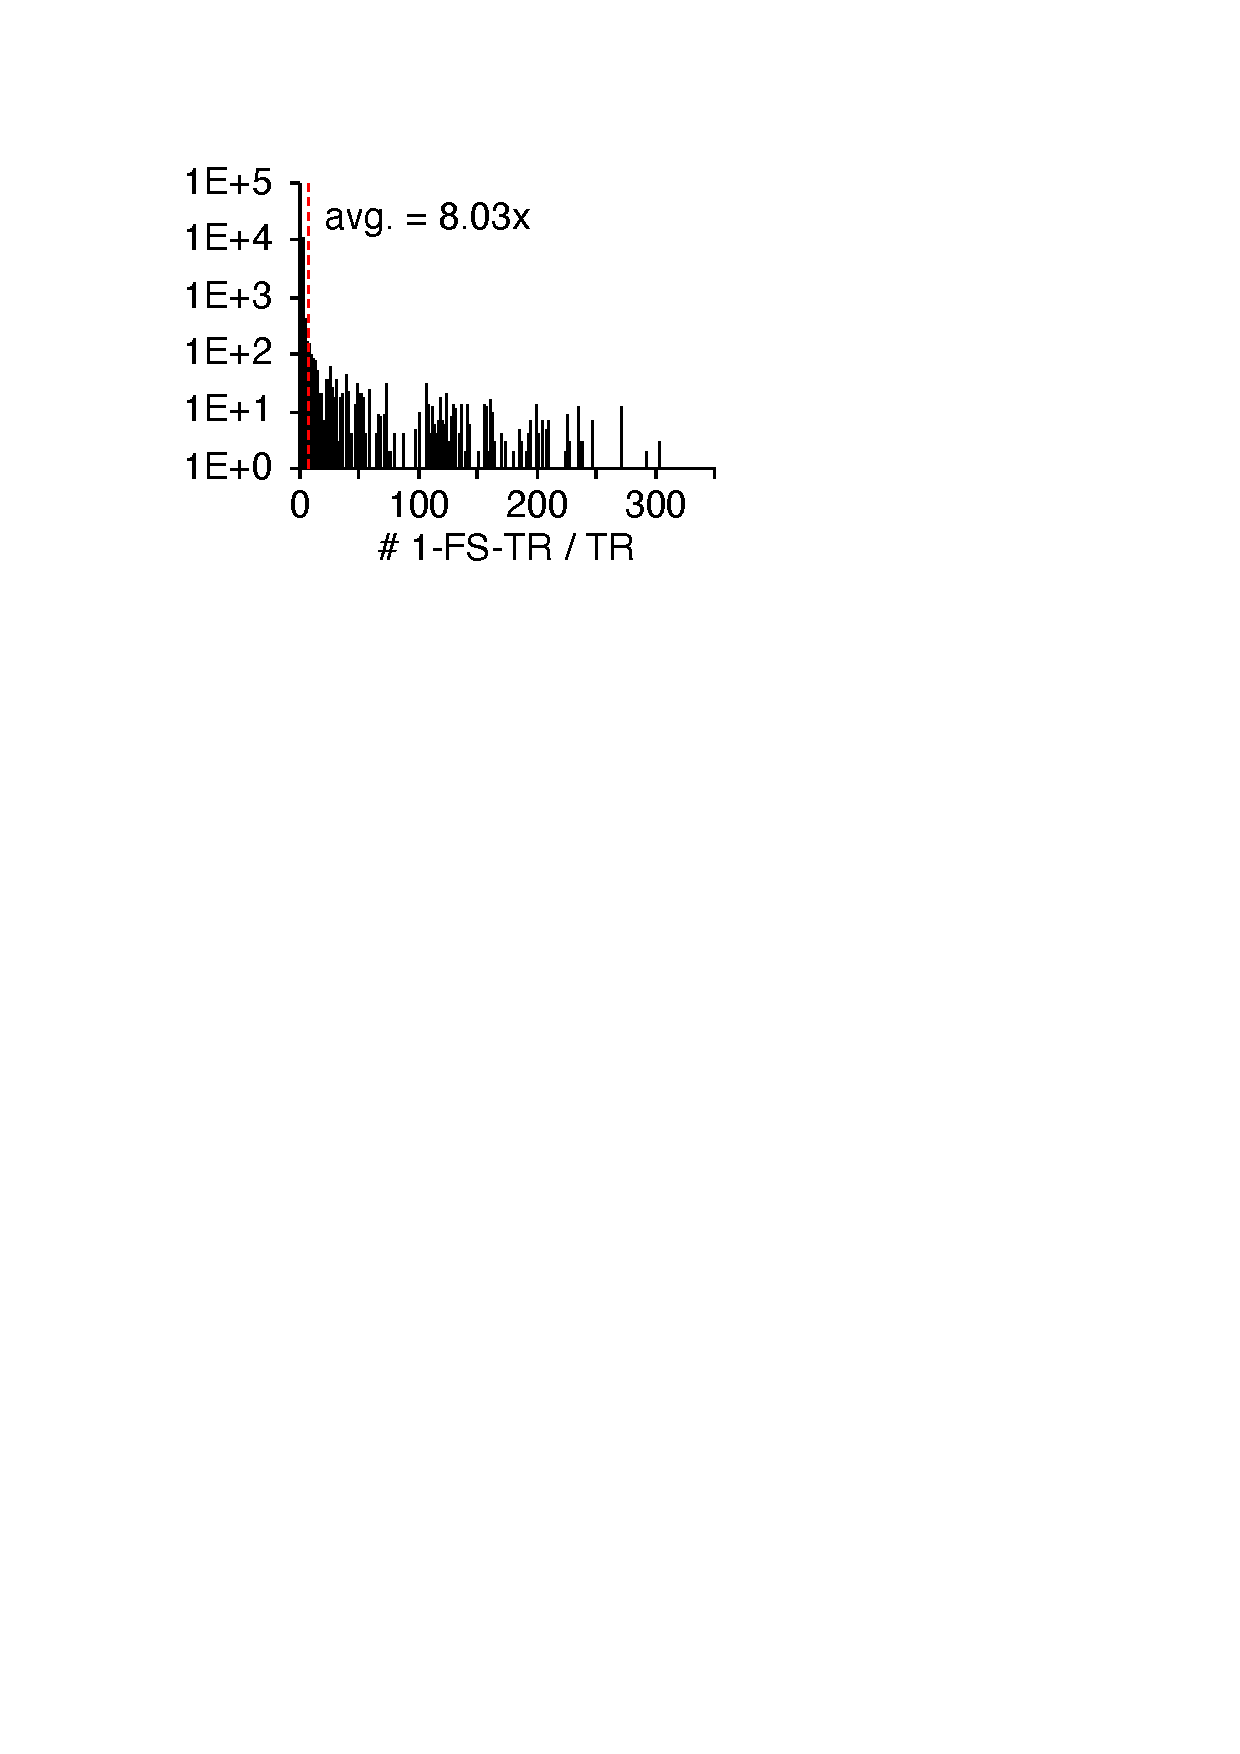
\includegraphics[width=\textwidth]{img/1-fs-hist}
    \subcaption{1-FS-TRs vs base TR}
  \end{subfigure}
  \begin{subfigure}{0.24\textwidth}
    \centering
    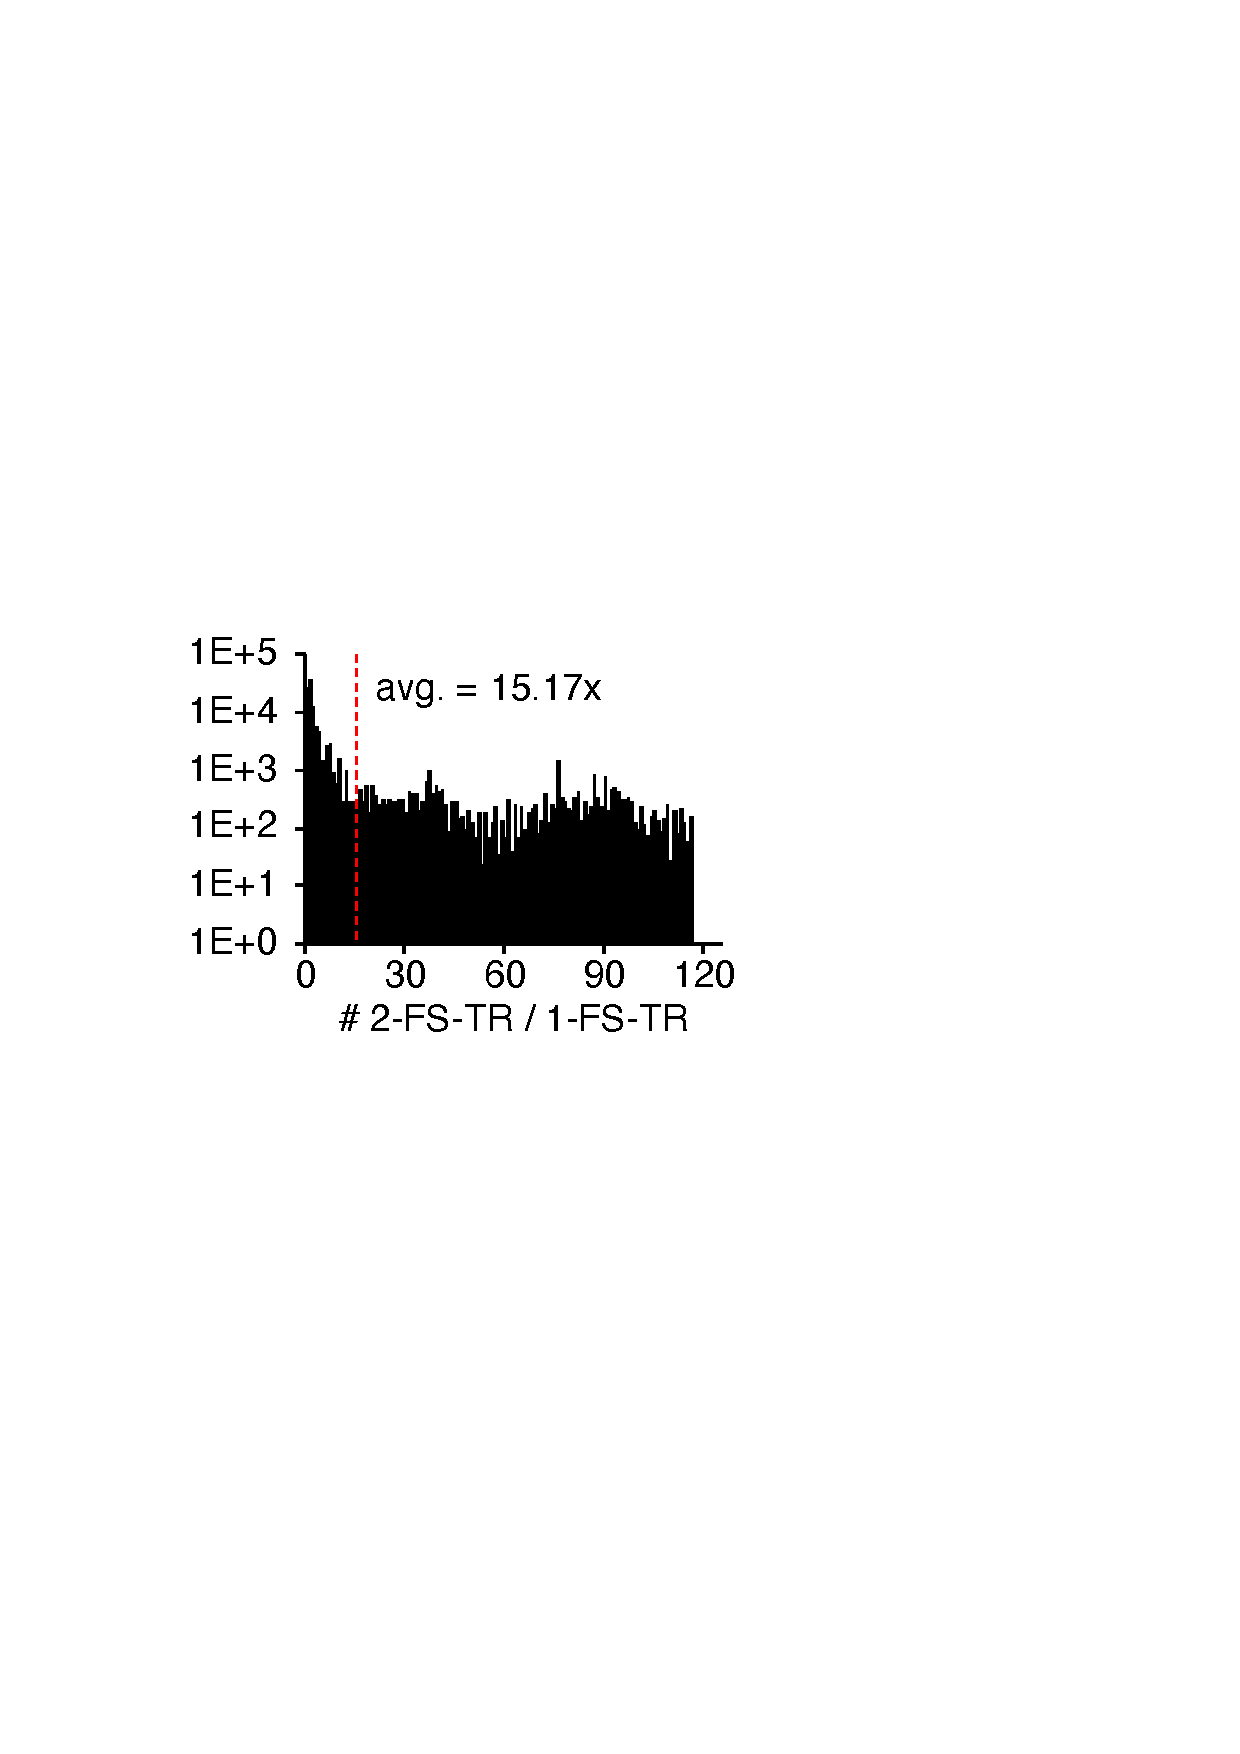
\includegraphics[width=\textwidth]{img/2-fs-hist}
    \subcaption{2-FS-TRs vs 1-FS-TR}
  \end{subfigure}
  \begin{subfigure}{0.24\textwidth}
    \centering
    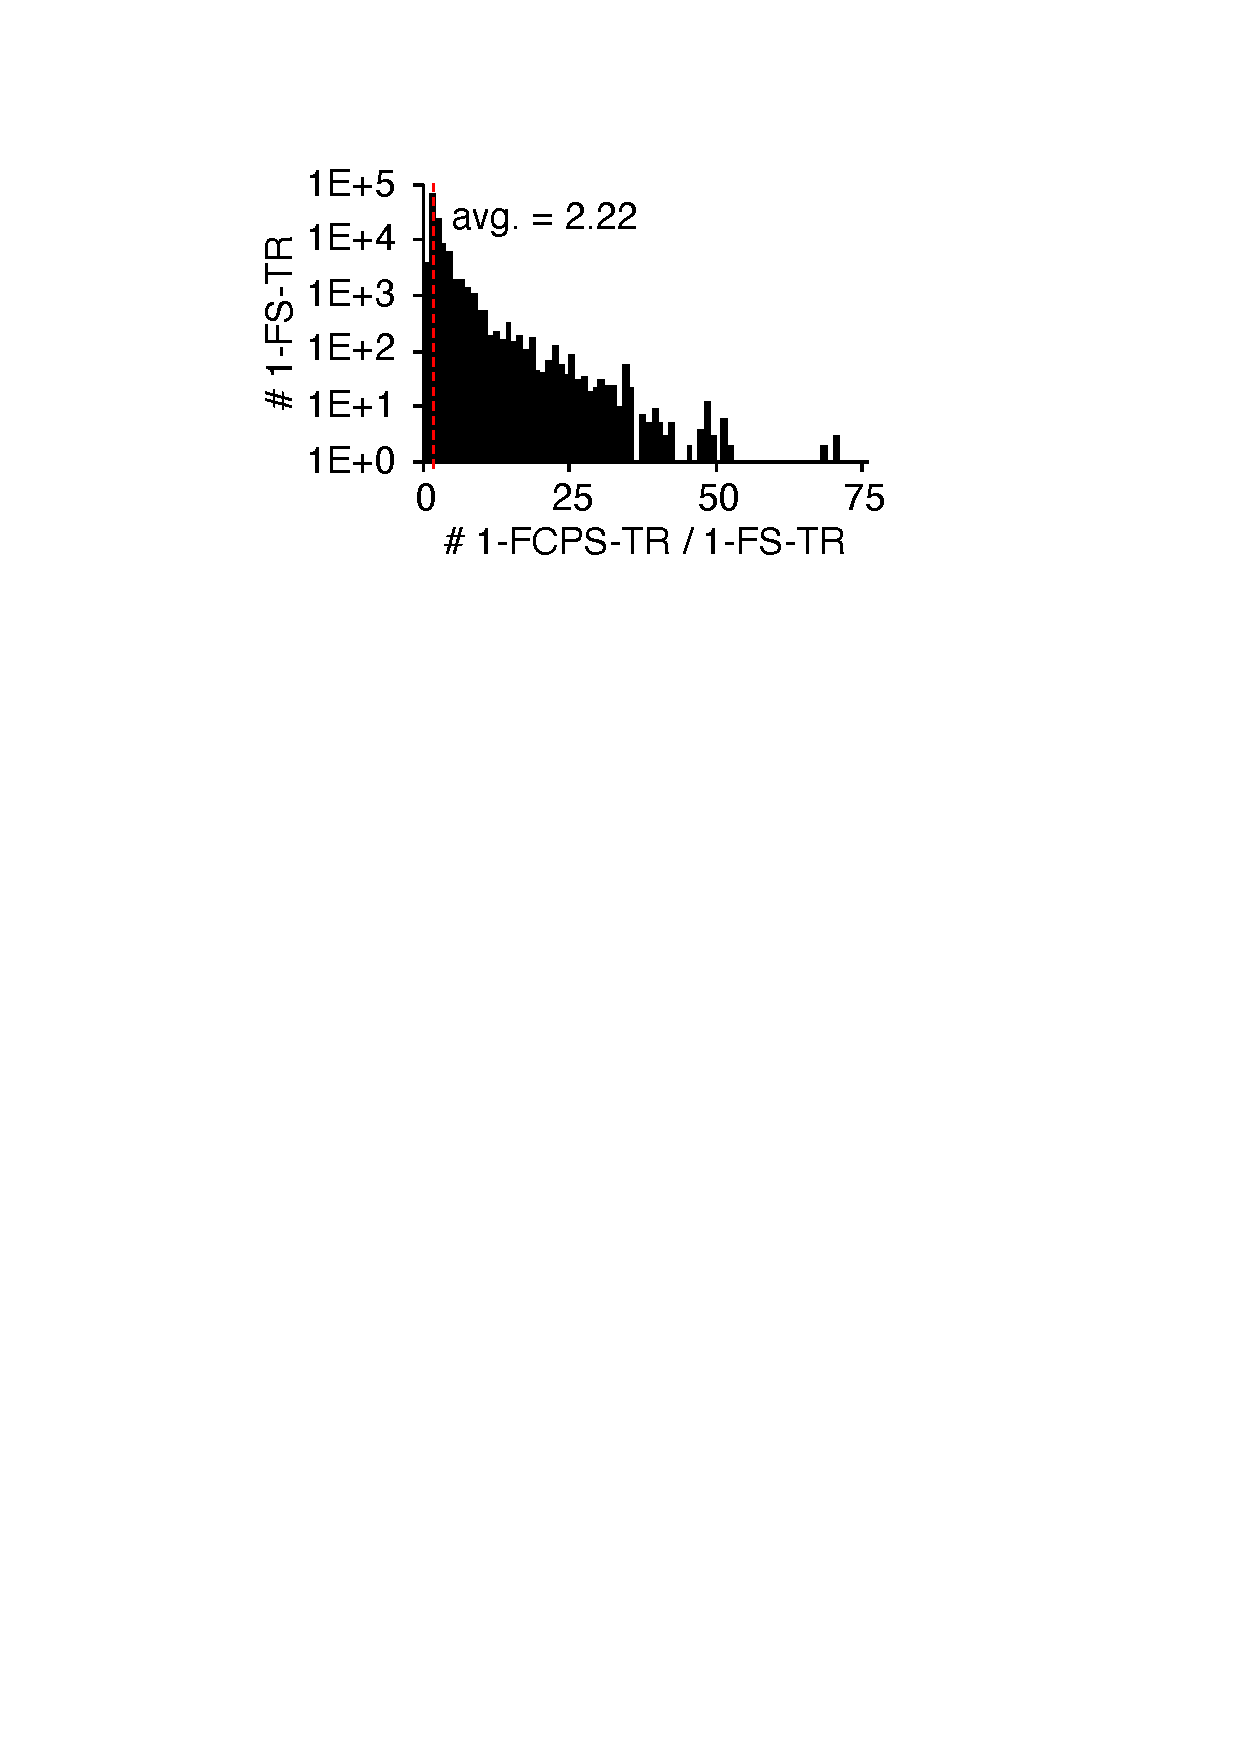
\includegraphics[width=\textwidth]{img/1-fcps-hist}
    \subcaption{1-FCPS-TRs vs 1-FS-TR}
  \end{subfigure}
  \begin{subfigure}{0.24\textwidth}
    \centering
    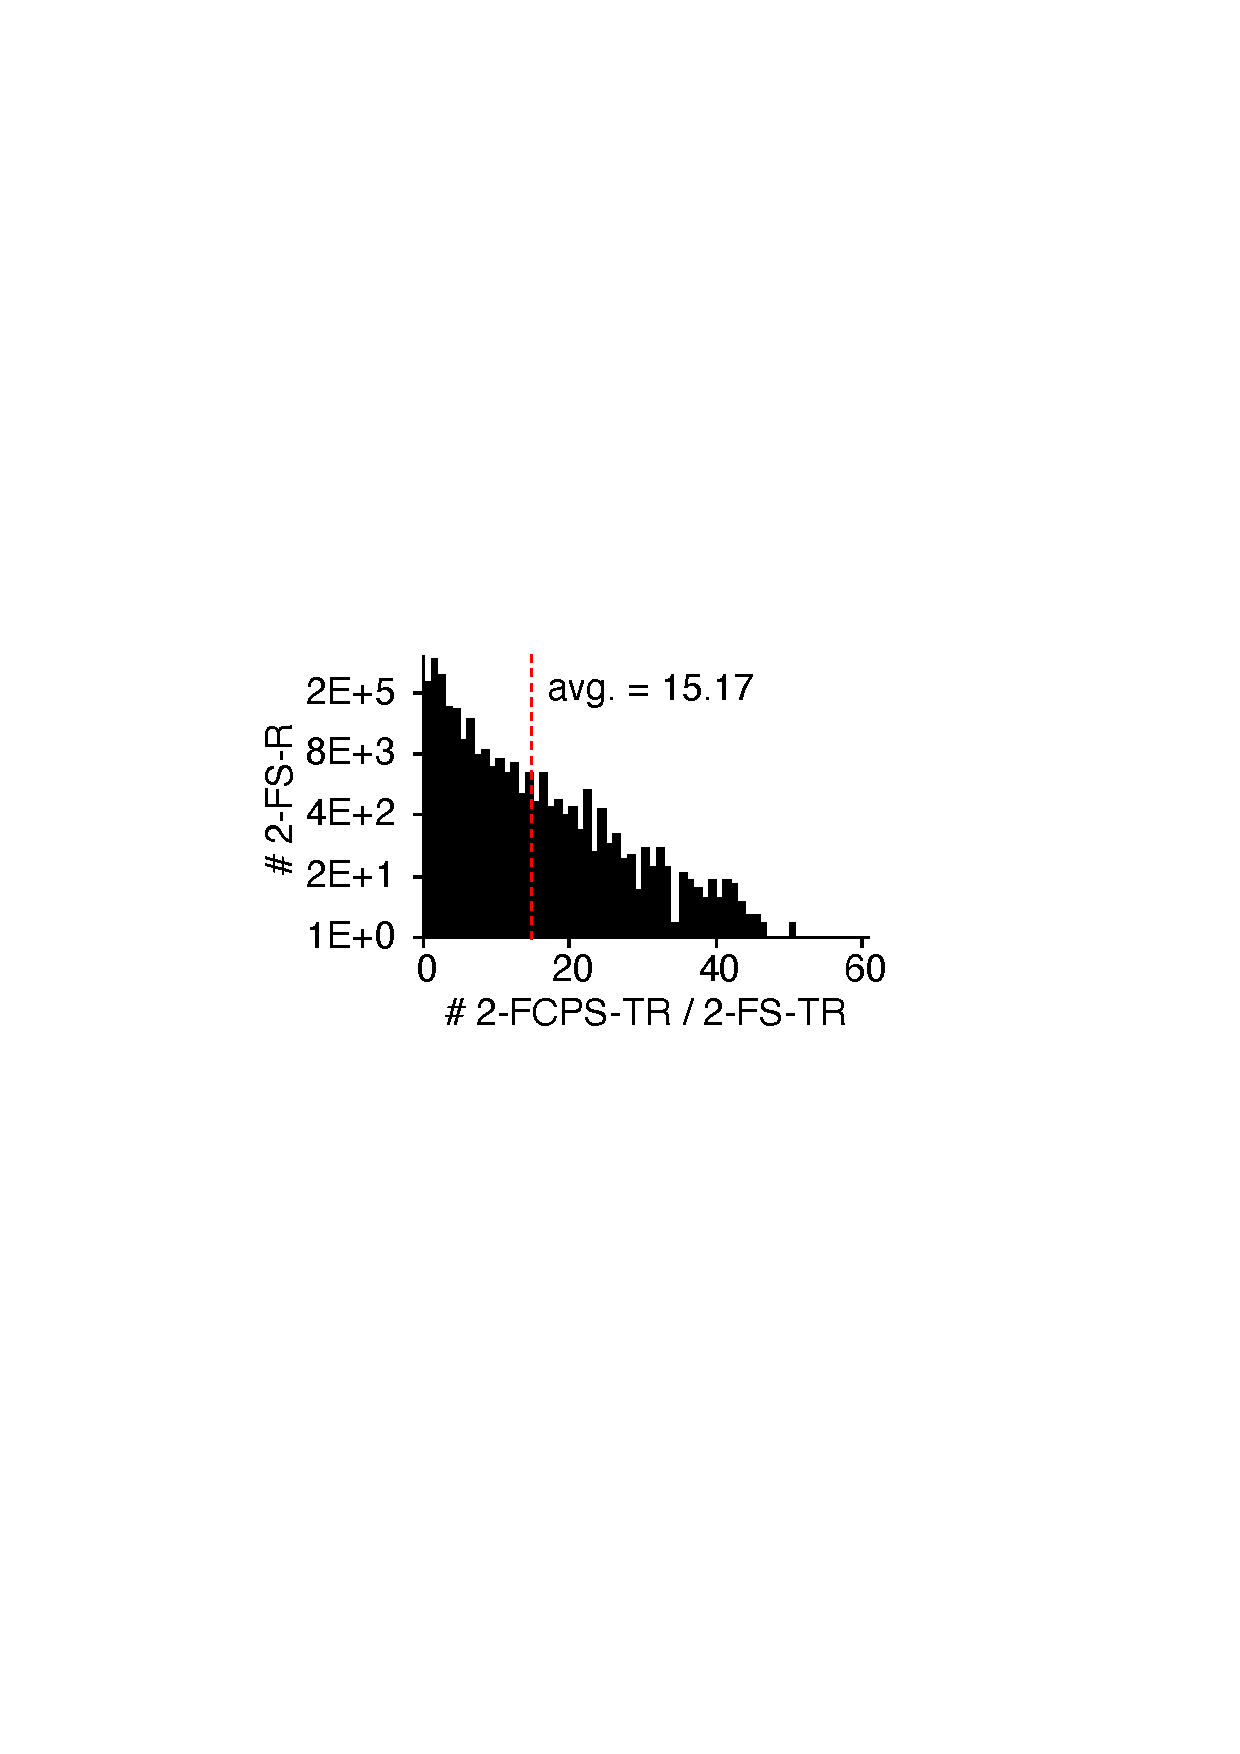
\includegraphics[width=\textwidth]{img/2-fcps-hist}
    \subcaption{2-FCPS-TRs vs 2-FS-TR}
  \end{subfigure}
  \caption{
    The histogram of numbers of $k$-FS or $k$-FCPS TRs per less sensitive $k$-FS
    or $k$-FCPS TR
  }
  \label{fig:hist}
\end{figure}

%----------------------------------------%

We also evaluate the effectiveness of $k$-FCPS coverage criteria compared to $k$-FS
coverage criteria.
%
According to Table~\ref{tab:compare}, the number of covered 1-FCPS- and
2-FCPS-TRs are 277.3K and 3,620.7K, respectively.
%
Thus, 2.22 (277.3K / 125.0K) 1-FCPS-TRs exist per each 1-FS-TR, and 1.91
(3,620.7K / 1,896.1K) 2-FCPS-TRs exist per each 2-FS-TR on average.
%
It means that 2.22 and 1.91 feature-call-paths exist from the innermost
language features to nodes or branches in each 1-FS-TR and 2-FS-TR,
respectively.
%
For a more detailed information, we also draw a histogram of the number of
covered 1-FCPS-TRs (or 2-FCPS-TRs) per each covered 1-FS-TR (or 2-FS-TR) in
Figures~\ref{fig:hist} (c) and (d).
%
The largest number of covered 1-FCPS-TRs per 1-FS-TR is 70 for a node
in the \jscode{Array.prototype.splice} built-in method.
%
It is a powerful built-in API feature that changes the contents of an array by
removing or replacing existing elements and/or adding new elements in place.
%
Thus, its semantics is quite complex and uses diverse helper functions, and the
number of possible feature-call-paths in this featuere is much larger than
the others.
%
The largest number of 2-FCPS-TRs per 2-FS-TR is 53 for a node whose
innermost enclosing feature is a syntactic feature for \jscode{yield} expressions
because it touches various helper functions for asynchronous behaviors.
%
Because of the increased number of TRs, the number of synthesized tests also
increased 1.34x (9,092 / 6,766) from 1-FS to 1-FCPS coverage criteria and 1.26x
(122,589 / 97,423) from 2-FS to 2-FCPS coverage criteria.
%
In addition, the number of detected unique bugs also increased when using
$k$-FCPS coverage criteria than $k$-FS coverage criteria.
%
The conformance tests synthesized with 1-FCPS and 2-FCPS coverage criteria
detected 4 (87 - 83) and 9 (111 - 102) more conformance bugs than
1-FS and 2-FS coverage criteria, respectively.
%
Now, we introduce a conformance bug example that show the effectiveness of $k$-FCPS
coverage criteria compared to the $k$-FS coverage criteria.

%----------------------------------------%

\paragraph{\textbf{\jscode{String.prototype.normalize}}}
%
The \jscode{String.prototype.normalize} built-in API normalizes a given string
into the normalization form named by a given argument.
%
For example, \jscode{"abc".normalize("NFC")} produces the NFC normalization form
of \jscode{"abc"}.
%
If an invalid name, such as an empty string \jscode{""}, is given as the
argument, it should throw a \textbf{RangeError} exception.
%
However, the following program noramlly terminates in GraalJS:
\begin{lstlisting}[style=JS, basicstyle=\footnotesize\ttfamily]
    String.prototype.normalize.call(0, ""); // Expected: RangeError
\end{lstlisting}
As we discussed in Section~\ref{sec:intro},
$k$-FS coverage criteria even with a high $k$ value cannot detect this bug,
while 1-FCPS and 2-FCPS coverage criteria can.


%----------------------------------------%
%----------------------------------------%

\subsection{Comparison with Test262}\label{sec:compare-test262}

\begin{figure}
  \centering
%
  \begin{subfigure}{0.49\textwidth}
    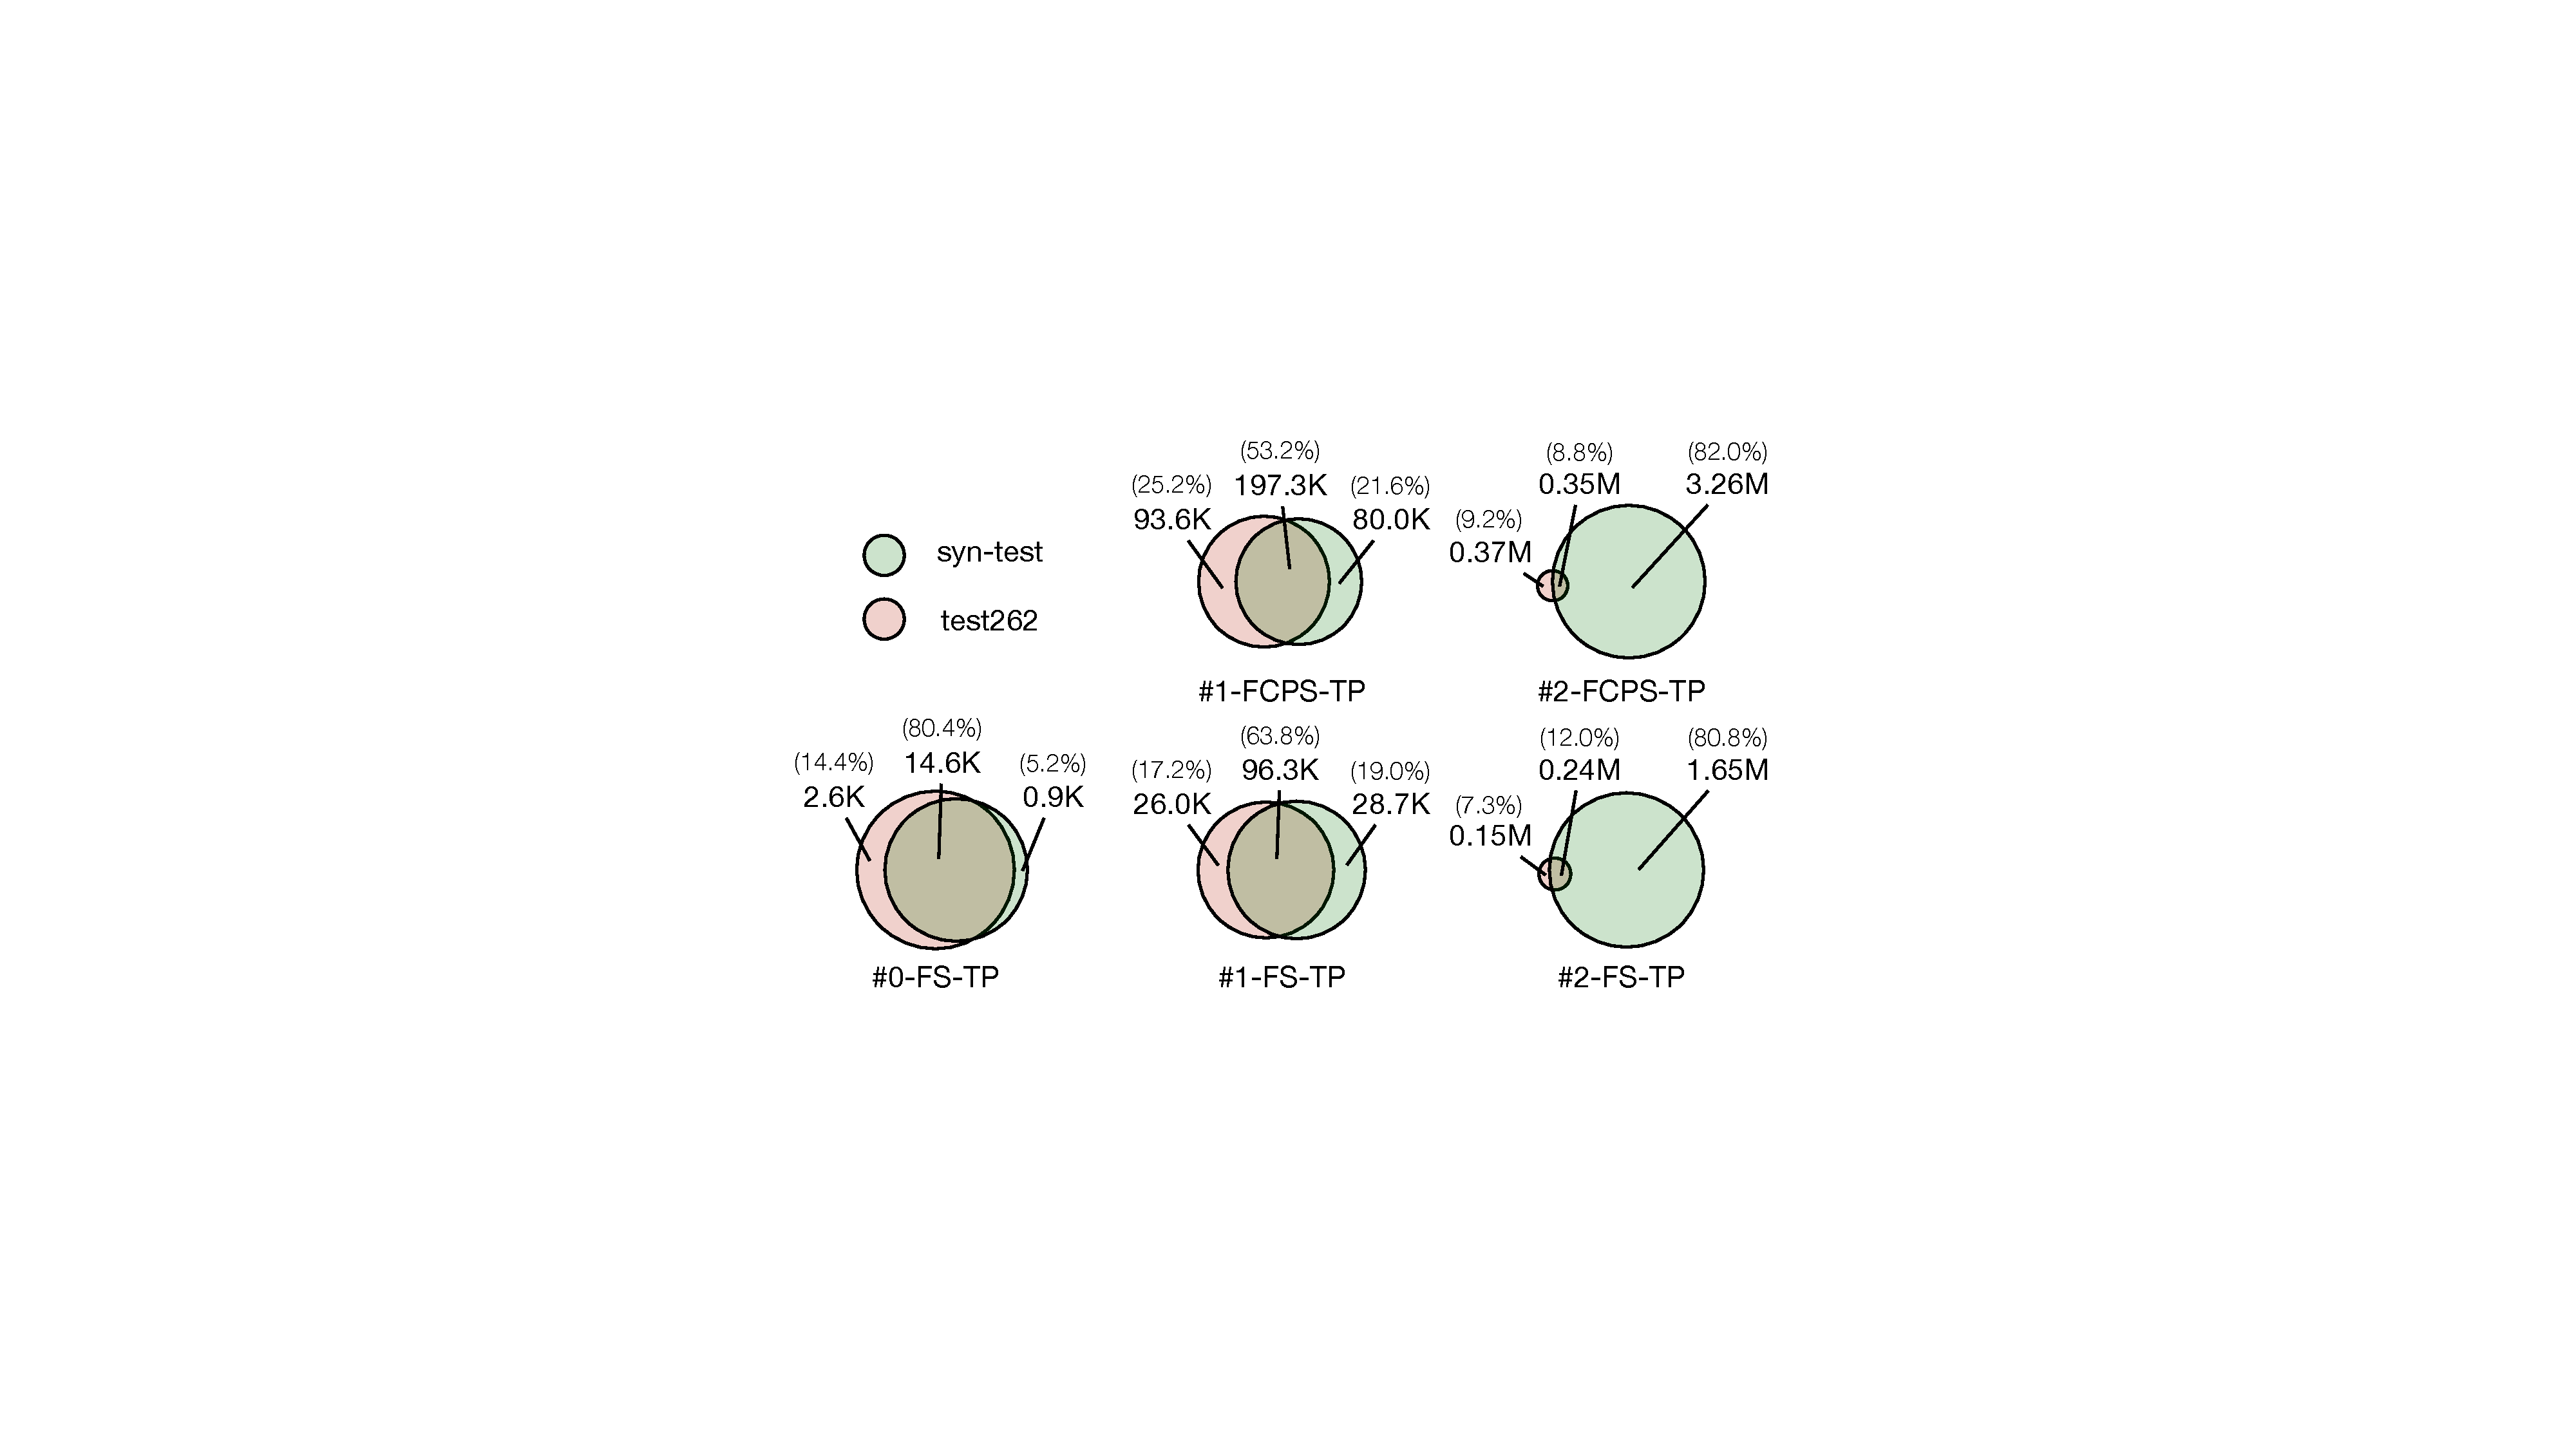
\includegraphics[width=\textwidth]{img/test262-venn}
    \caption{Covered TRs by synthesized tests and Test262}
  \end{subfigure}
%
  \begin{subfigure}{0.49\textwidth}
    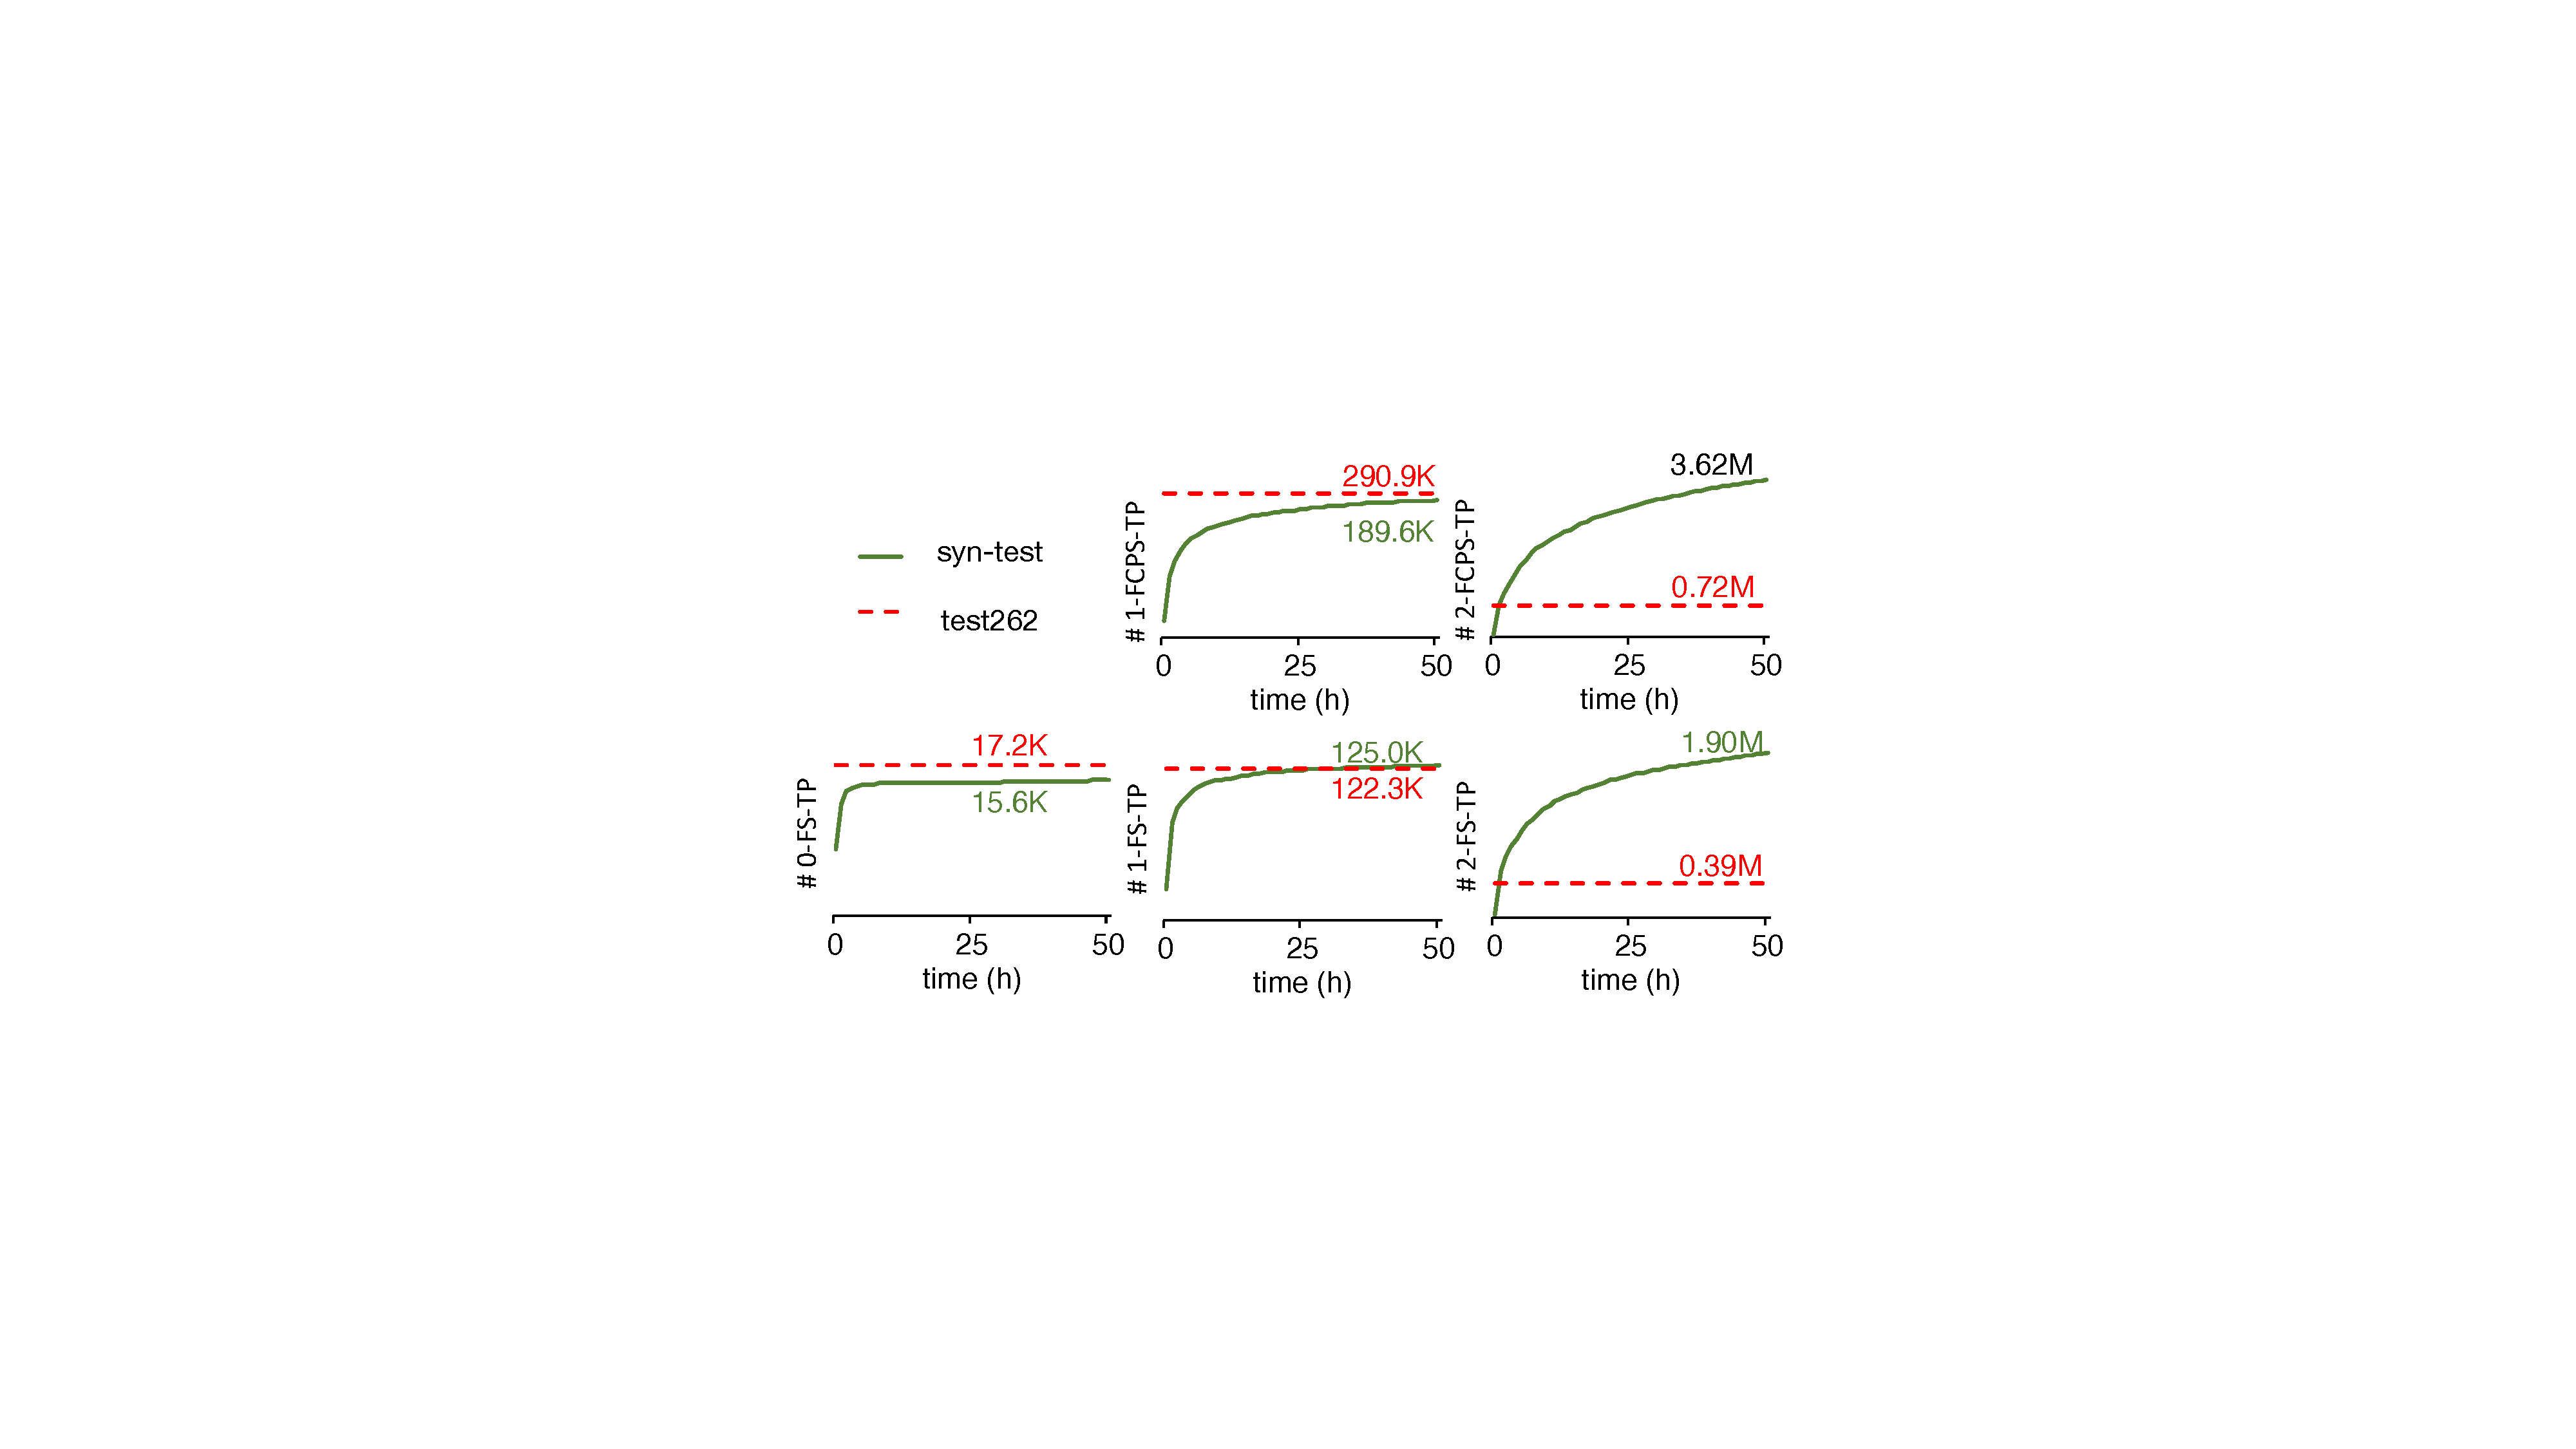
\includegraphics[width=\textwidth]{img/test262-time}
    \caption{Covered TRs over time}
  \end{subfigure}
%
  \caption{Covered $k$-FS-TRs and $k$-FCPS-TRs for synthesized tests via $\tool$ and Test262
  }
  \label{fig:test262}
\vspace*{-1em}
\end{figure}

%----------------------------------------%

We compare the coverage of automatically synthesized conformance tests with that
of Test262, the official JavaScript conformance test suite.
As described in Section~\ref{sec:impl}, the baseline tool $\jest$ relies on the
mechanized specification extracted by $\esmeta$.
Thus, we filter out conformance tests in Test262 that utilize language
features not supported in the extracted mechanized specification.
We use the conventional methodology in the literature~\cite{kjs, jiset, javert}
to remove inapplicable tests in Test262.
Then, we measured the coverage of 23,910 applicable Test262 conformance tests
with five $k$-FS and $k$-FCPS node-or-branch coverage criteria.


Figure~\ref{fig:test262} shows
(b) venn diagrams of
the numbers of covered $k$-FS-TRs and 
$k$-FCPS-TRs for the synthesized conformance tests (\sname{syn-test}) via
$\tool$ and applicable conformance tests in Test262 (\sname{test262}) and
(b) their changes over time.
Without any feature-sensitive coverages, the coverage of synthesized tests is
less than that of Test262, and only 5.2\% (0.9K) 0-FS-TRs are newly covered by
the synthesized tests.
%
On the other hand, the numbers of $k$-FS-TRs covered by only synthesized tests
increase when using higher $k$: 28.7K (19.0\%) for 1-FS-TRs and 1.65M (80.8\%)
for 2-FS-TRs.
%
In addition, the number of 1-FCPS-TRs (or 2-FCPS-TRs) covered by only
synthesized tests is higher than the number of 1-FS-TRs (or 2-FS-TRs)
covered by only synthesized tests:
80.0K (21.6\%) for 1-FCPS-TRs and 3.26M (82.0\%) for 2-FCPS-TRs.
Figure~\ref{fig:test262}(b) also shows that the coverage of Test262 is
better than that of synthesized tests without any feature-sensitive
coverages, but the coverage of synthesized tests outperforms that of
Test262 with $2$-FS-TRs and $2$-FCPS-TRs.
%
We believe that this is why $\tool$ successfully detected diverse new bugs in
existing JavaScript implementations, even though they have been heavily tested
using Test262 and various fuzzing techniques.
